\documentclass{beamer}

\usetheme{Warsaw}
%\usetheme{CambridgeUS}

% modification history
% created on 18 sep 2011
% modified on 25 mar

%\usepackage{amsfonts, amsmath, amssymb}

%\setbeamertemplate{theorems}[numbered]
%\setbeamertemplate{theorems}[ams style] 
\usepackage[skins,breakable]{tcolorbox}
%\usepackage[normalem]{ulem}

%\usefonttheme[onlymath]{serif}                     // change the style of math font 

%=============set slide number=================
\addtobeamertemplate{navigation symbols}{}{
    \usebeamerfont{footline}
    \usebeamercolor[fg]{footline}
    \hspace{1em}
    \insertframenumber/\inserttotalframenumber
}
\setbeamercolor{footline}{fg=black}
\setbeamerfont{footline}{series=\bfseries}


%=============set footline=====================
\setbeamertemplate{footline}
{
  \leavevmode%
  \hbox{%
  \begin{beamercolorbox}[wd=.55\paperwidth,ht=2.25ex,dp=1ex,center]{author in head/foot}%
    \usebeamerfont{author in head/foot}\insertshortauthor
  \end{beamercolorbox}%
  \begin{beamercolorbox}[wd=.45\paperwidth,ht=2.25ex,dp=1ex,center]{title in head/foot}%
    \usebeamerfont{title in head/foot}\insertshorttitle
  \end{beamercolorbox}}%
  \vskip0pt%
}

%creating a rectangle box def
\newtcbox{\mybox}[1][red]{arc=0pt,outer arc=0pt,colback=#1!10!white,colframe=#1!50!black, boxsep=0pt,left=1pt,right=1pt,top=2pt,bottom=2pt,boxrule=0pt,bottomrule=1pt,toprule=1pt}

\newtcbox{\xmybox}[1][red]{arc=7pt,colback=#1!10!white,colframe=#1!50!black,before upper={\rule[-3pt]{0pt}{10pt}},boxrule=1pt,boxsep=0pt,left=6pt,right=6pt,top=2pt,bottom=2pt}
%the ``on line'' option doesn't work. so omitting it

%===== spacing =====

\def\extraspacing{\vspace{2mm} \noindent}
\def\vgap{\vspace{2mm}}
\def\hgap{\textrm{\hspace{1mm}}}

%===== tabbing =====

\def\tab{\hspace{2mm}}
\def\tabpos{\hspace{4mm} \= \hspace{4mm} \= \hspace{4mm} \= \hspace{4mm} \=
\hspace{4mm} \= \hspace{4mm} \= \hspace{4mm} \= \hspace{4mm} \= \hspace{4mm}
\kill}
\newcommand{\mytab}[1]{\begin{tabbing}\tabpos #1\end{tabbing}}

%===== blocks =====

% \newtheorem{theorem}{Theorem}
% \newtheorem{lemma}{Lemma}
% \newtheorem{corollary}{Corollary}
% \newtheorem{proposition}{Proposition}
% \newtheorem{definition}{Definition}
% \newtheorem{problem}{Problem}

\newcommand{\cbox}[2]{\begin{tcolorbox}[arc=0mm, colframe=#1!50!black, colback=#1!10!white]#2\end{tcolorbox}}
\newcommand{\minipg}[2]{\begin{center}\begin{minipage}{#1}#2\end{minipage}\end{center}}
\newcommand{\myfrm}[1]{\begin{frame}\begin{small}#1\end{small}\end{frame}} 
\newcommand{\myitems}[1]{\begin{itemize}#1\end{itemize}}
\newcommand{\myenums}[1]{\begin{enumerate}#1\end{enumerate}}
\newcommand{\myfig}[1]{\begin{figure}\centering #1\end{figure}}
    
%===== math macros =====
\newcommand{\bm}[1]{\textrm{\boldmath${#1}$}}
%\newcommand{\smat}[2]{\left[\begin{tabular}{#1}#2\end{tabular}\right]}
%\newcommand{\bmat}[2]{\left|\begin{tabular}{#1}#2\end{tabular}\right|}
\newcommand{\bmat}[1]{\begin{bmatrix}#1\end{bmatrix}}
\newcommand{\vmat}[1]{\begin{vmatrix}#1\end{vmatrix}}
\newcommand{\myeqn}[1]{\begin{eqnarray}#1\end{eqnarray}}
\newcommand{\set}[1]{\{#1\}}

\def\eps{\epsilon}
\def\fr{\frac}
\def\lc{\lceil}
\def\lf{\lfloor}
\def\rc{\rceil}
\def\rf{\rfloor}
\def\Pr{\textrm{\boldmath$Pr$}}
\def\expt{\textrm{\boldmath$E$}}
\def\real{\mathbb{R}}
\def\int{\mathbb{Z}}
\def\*{\star}
\def\tO{\tilde{O}}

\DeclareMathOperator*{\argmin}{arg\,min}
\DeclareMathOperator*{\polylg}{polylg}
\DeclareMathOperator*{\polylog}{polylog}
\DeclareMathOperator*{\intr}{\cap}

\def\nn{\nonumber}
\def\mit{\mathit}


%===== misc =====

\def\done{\hspace*{\fill} $\framebox[2mm]{}$}	% end of proof
\def\ttt{\texttt}

%===== coloring =====
\newcommand{\red}[1]{\textcolor{red}{#1}}
\newcommand{\bred}[1]{\textcolor{red}{\bf #1}}
\newcommand{\blue}[1]{\textcolor{blue}{\bf #1}}

\usepackage{color}
\usepackage{graphicx}
\usepackage{multirow}
\usepackage{wrapfig}
\usepackage[skins,breakable]{tcolorbox}

\def\done{\hfill$\square$}
\def\ttt{\texttt}
\def\vgap{\vspace{5mm}}

\def\sort{\mit{sort}}

\title[DATABASE SYSTEM PRINCIPLES]{Query Processing 3:\\ Sort Join}

\author[Yufei Tao @ NTU]{Yufei Tao}
\institute[]{\url{https://www.cse.cuhk.edu.hk/~taoyf}}
\date{}

% \def\dtm{\mathit{d\mbox{-}tm}}
% \def\ftm{\mathit{f\mbox{-}tm}}
\def\bestext{\mathit{best\mbox{-}ext}}

\begin{document}
%-------------------------------------------------------------
\begin{frame}
    \titlepage
%     \begin{tcolorbox}[arc=0mm, colframe=green!50!black, colback=green!10!white] 
%     \end{tcolorbox}
\end{frame}
%-------------------------------------------------------------
\begin{frame}
\begin{small}
    This lecture will introduce the \blue{sort join} algorithm for computing a natural join involving two relations.
    %\vgap
\end{small}    
\end{frame}
%-------------------------------------------------------------
\myfrm{
    \xmybox{The Binary Join Problem}

    \vgap

    $\red{R_1(X, Y)}$: A relation with attributes $X$ and $Y$. \\
    $\red{R_2(X, Z)}$: A relation with attributes $X$ and $Z$. \\
    $\red{B_1} =$ the number of disk blocks that $R_1$ occupies. \\
    $\red{B_2} =$ the number of disk blocks that $R_2$ occupies. \\
    $\red{M} =$ the number of memory blocks (a.k.a., the buffer blocks). \\
    \myitems{
        \item We assume $M \ge 3$.
    }

    \vgap

    \blue{Goal:} Compute the join result $R_1 \bowtie R_2$.

    \vgap

    We will carry out our discussion under another assumption: \\
    \cbox{red}{
        \blue{No skew assumption:} \\
        For any $X$-value, the tuples of $R_1$ having that $X$-value fit in at most $M-2$ blocks.
    }

}
%-------------------------------------------------------------
\myfrm{
    \xmybox{Sort Join}

    \vgap

    \blue{Step 1:} Sort $R_1(X, Y)$ on $X$, and sort $R_2(X, Z)$ on $X$ \\
    \myitems{
        \item Using the external sort algorithm.
    }
    \blue{Step 2:} Scan the sorted $R_1$ and $R_2$ synchronously to output the result.

    \vgap

    Next, we will explain how to do Step 2 in $B_1 + B_2$ I/Os.
}
%-------------------------------------------------------------
\myfrm{
    \xmybox{Sort Join: Step 2}

    %\vgap

    We will maintain a value $\red{x_1}$ for $R_1$ and a value $\red{x_2}$ for $R_2$ to enforce the following invariant:

    \cbox{blue}{
        \blue{Invariant:} All the result tuples of $R_1$ (resp., $R_2$) with $X$-values less than $x_1$ (resp., $x_2$) have been output.
    }

    %\vgap

    In the beginning, load the first blocks of $R_1$ and $R_2$ into memory. \\
    Set $x_1$ (resp., $x_2$) to the $X$-value of the first tuple of $R_1$ (resp., $R_2$).

    \begin{center}
        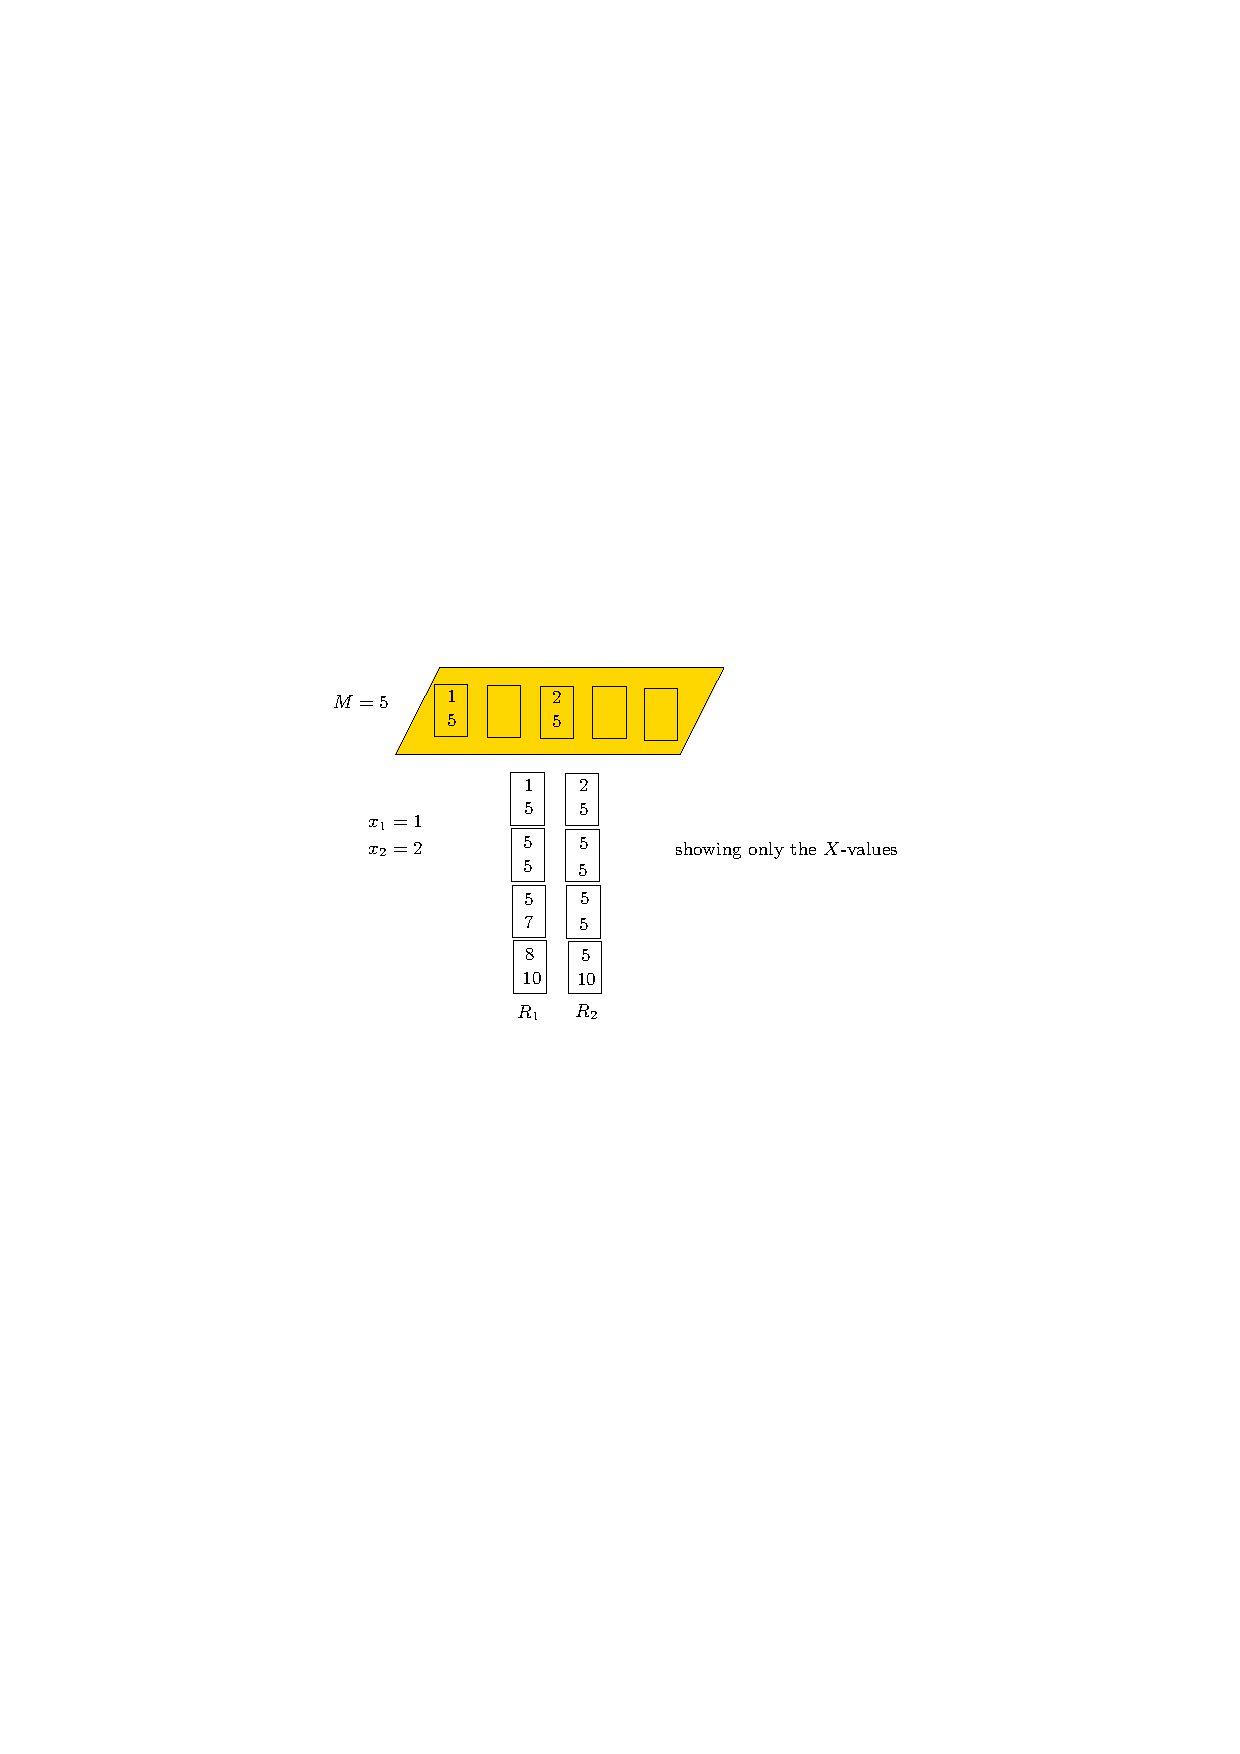
\includegraphics[height=40mm]{./artwork/em-sj1}
    \end{center}

}
%-------------------------------------------------------------
\myfrm{
    \xmybox{Sort Join: Step 2}

    \bred{If $x_1 < x_2$}, move $x_1$ to the next element of $R_1$ (loading the next block of $R_1$ into memory if necessary).
    \bred{If $x_2 < x_1$}, move $x_2$ to the next element of $R_2$ (loading the next block of $R_2$ into memory if necessary).

    \vgap

    \begin{center}
        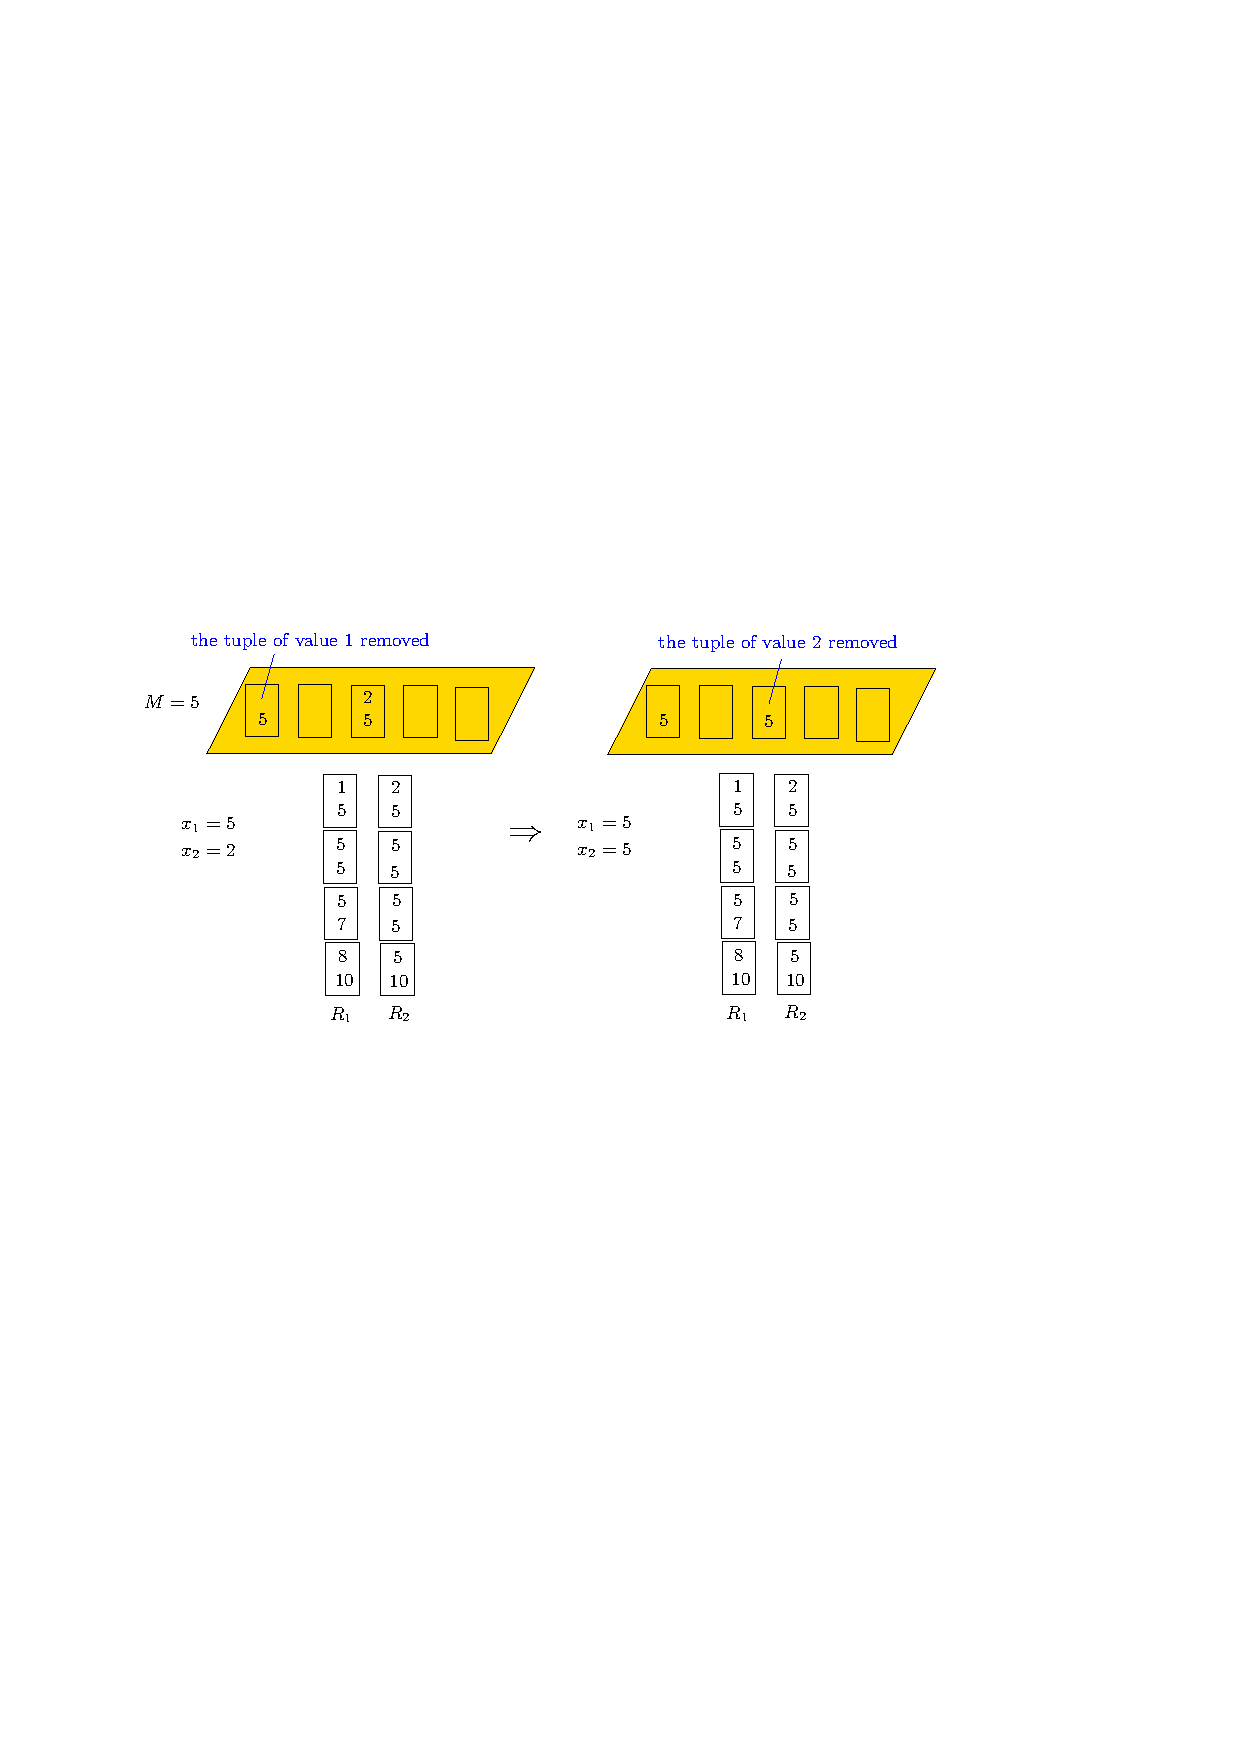
\includegraphics[height=40mm]{./artwork/em-sj2}
    \end{center}
}
%-------------------------------------------------------------
\myfrm{
    \xmybox{Sort Join: Step 2}

    \bred{If $x_1 = x_2$}, read into memory all tuples of $R_1$ with $X$-value equal to $x_1$. \\
    By the no-skew assumption, they occupy at most $M-2$ memory blocks.

    %\vgap

    \begin{center}
        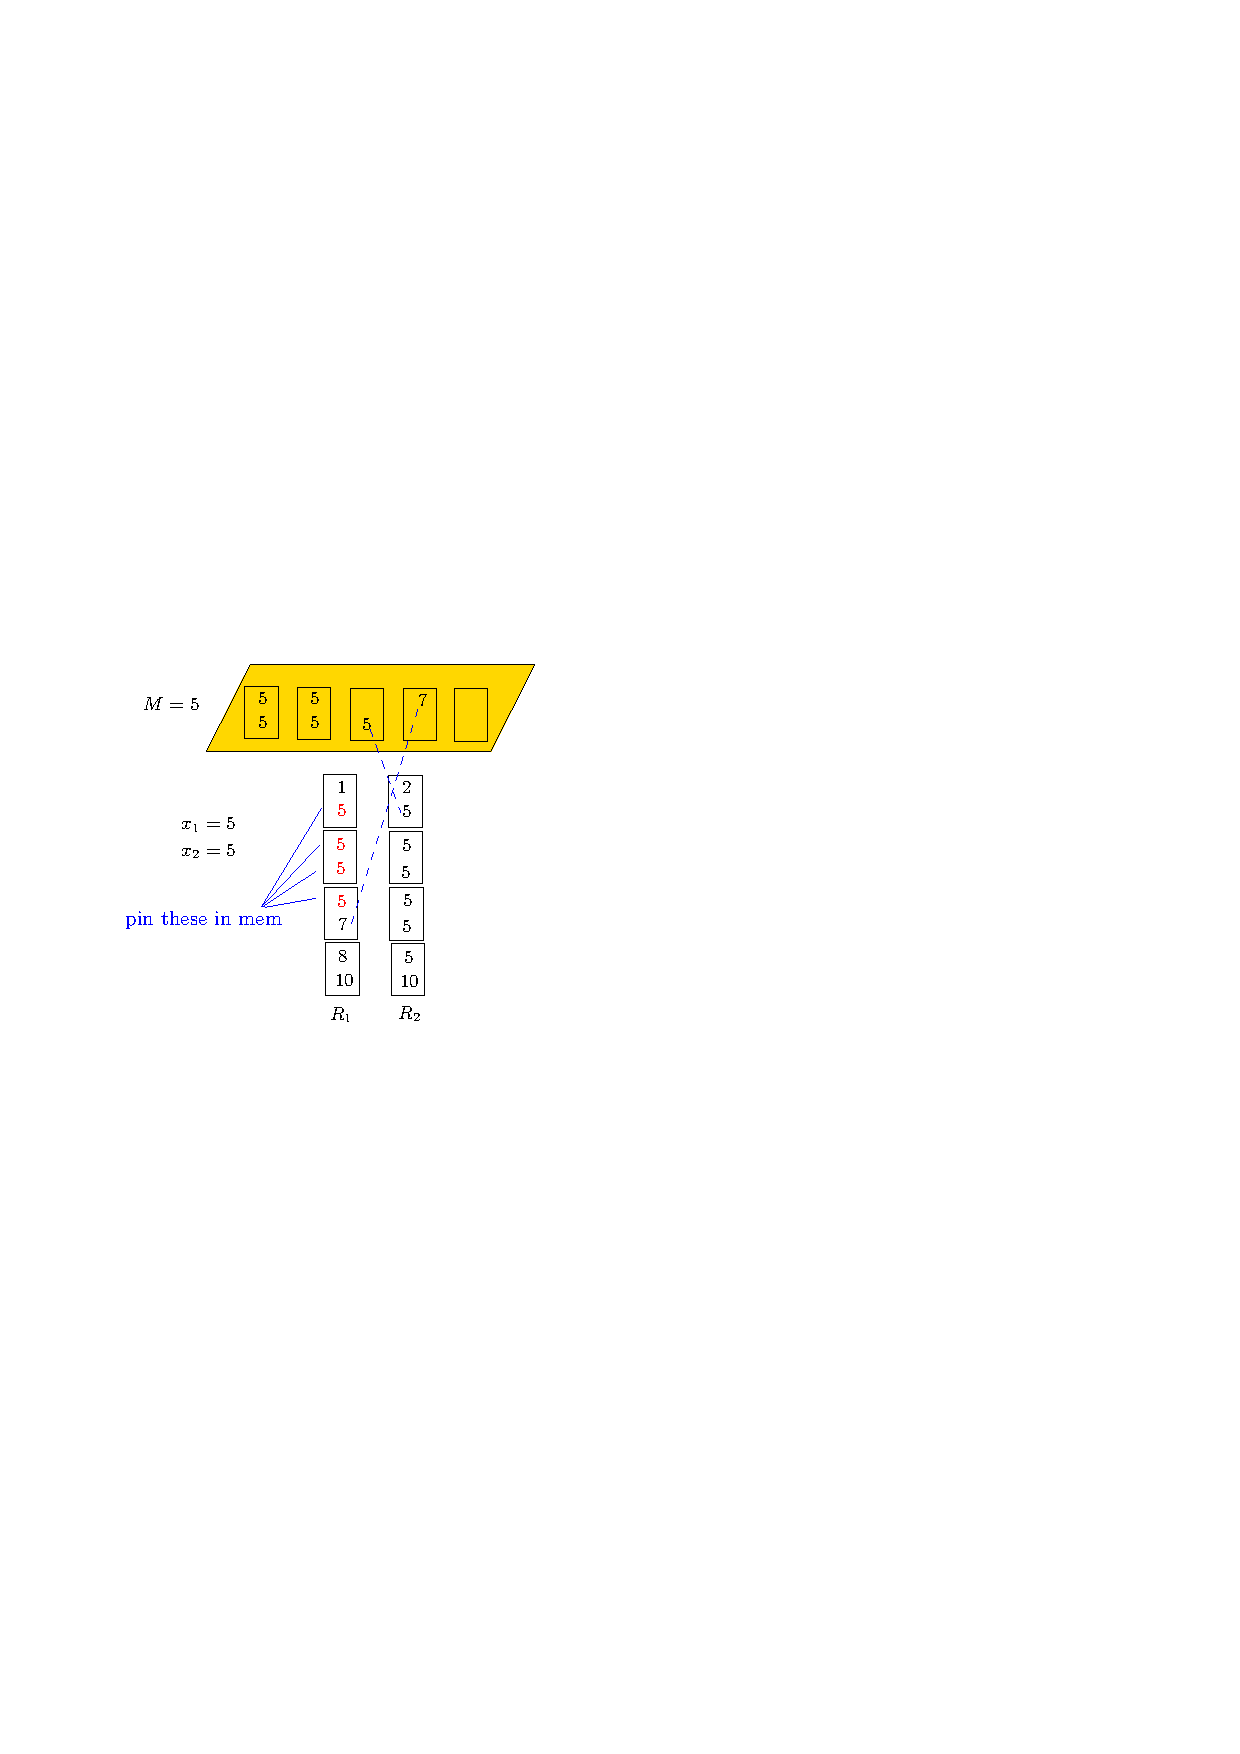
\includegraphics[height=40mm]{./artwork/em-sj3}
    \end{center}

}
%-------------------------------------------------------------
\myfrm{
    \xmybox{Sort Join: Step 2}

    Then use one memory block to read every block of $R_2$ containing tuples whose $X$-values equal $x_2$ (one block at a time). For each block read, produce all the result tuples whose $X$-values equal $x_2$.

    %\vgap

    \begin{center}
        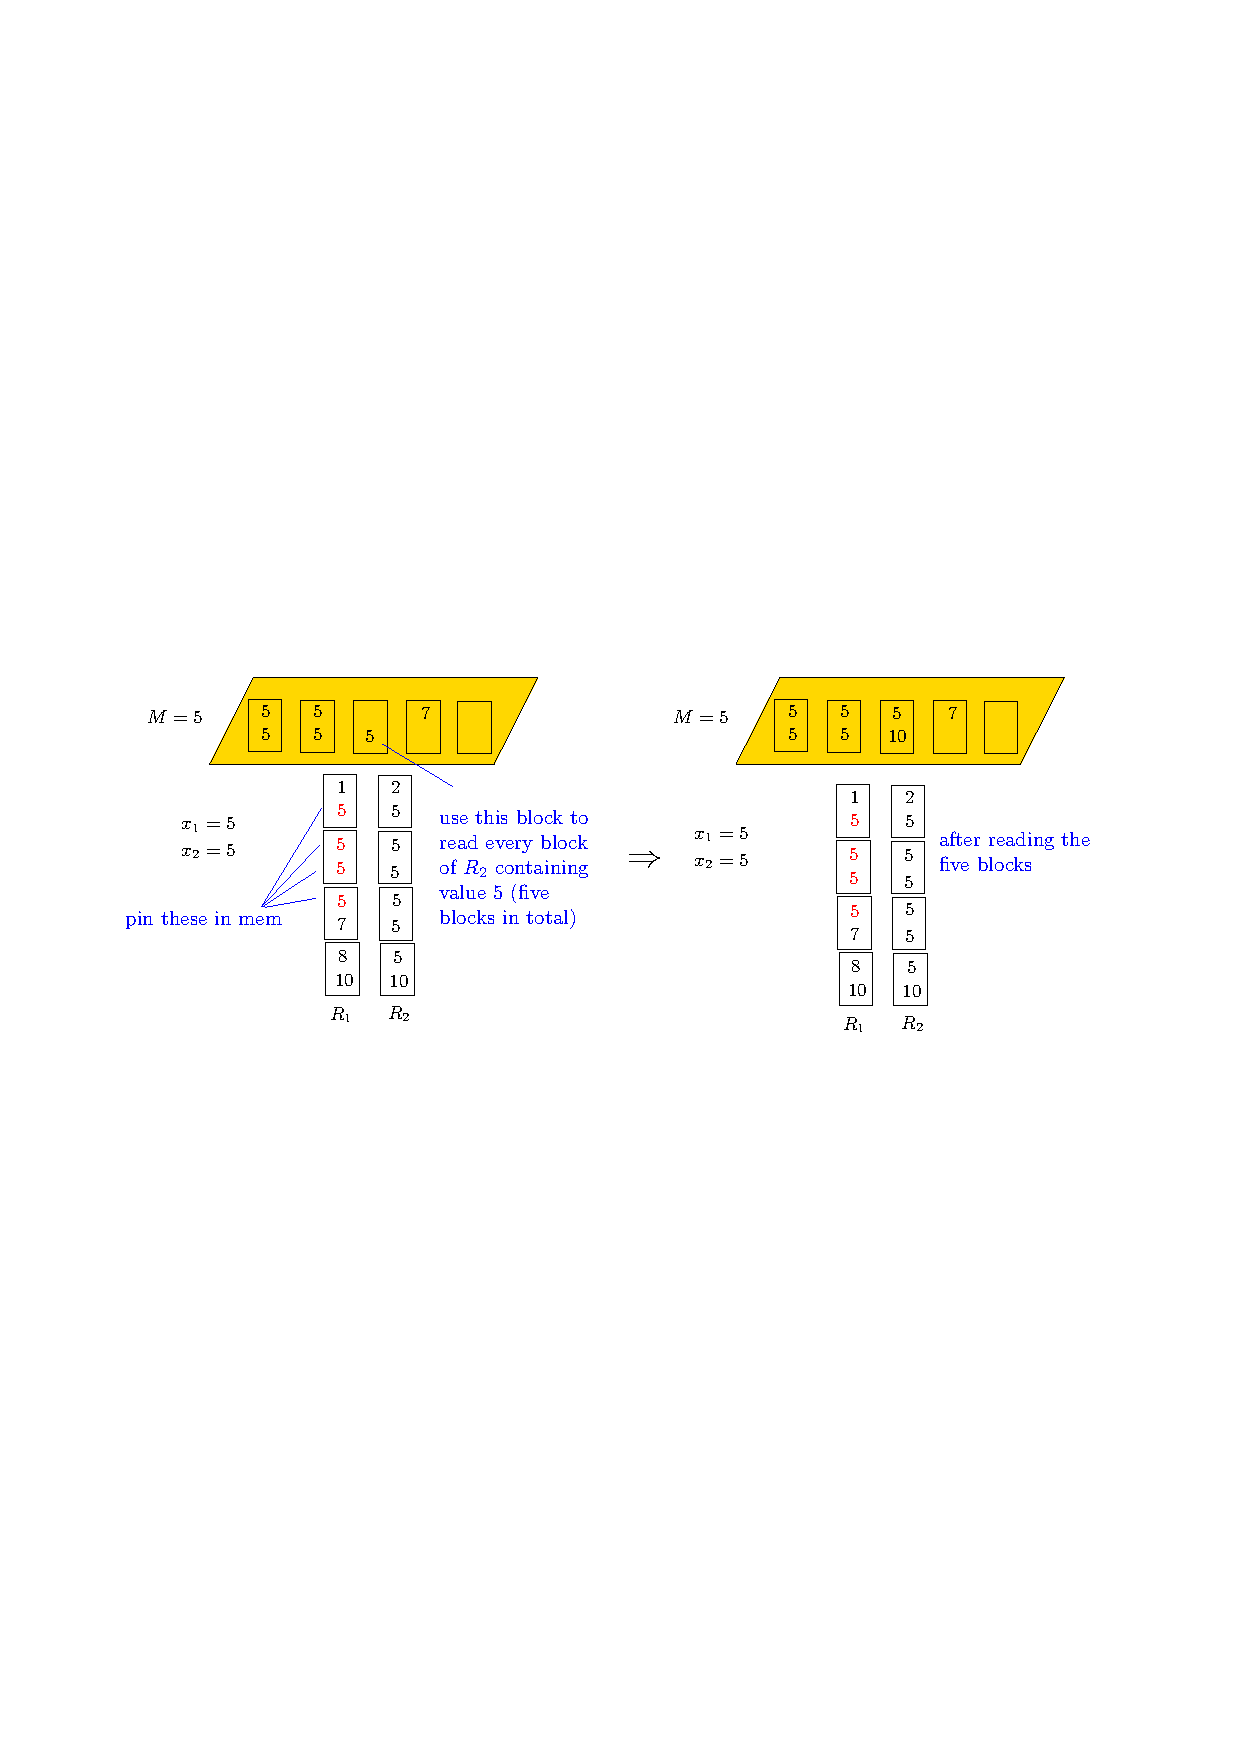
\includegraphics[height=40mm]{./artwork/em-sj4}
    \end{center}


}
%-------------------------------------------------------------
\myfrm{
    \xmybox{Sort Join: Step 2}

    Move $x_1$ to the next element of $R_1$ (reading the next block of $R_1$ if necessary). Move $x_2$ to the next element of $R_2$ (reading the next block of $R_2$ if necessary).

    %\vgap

    \begin{center}
        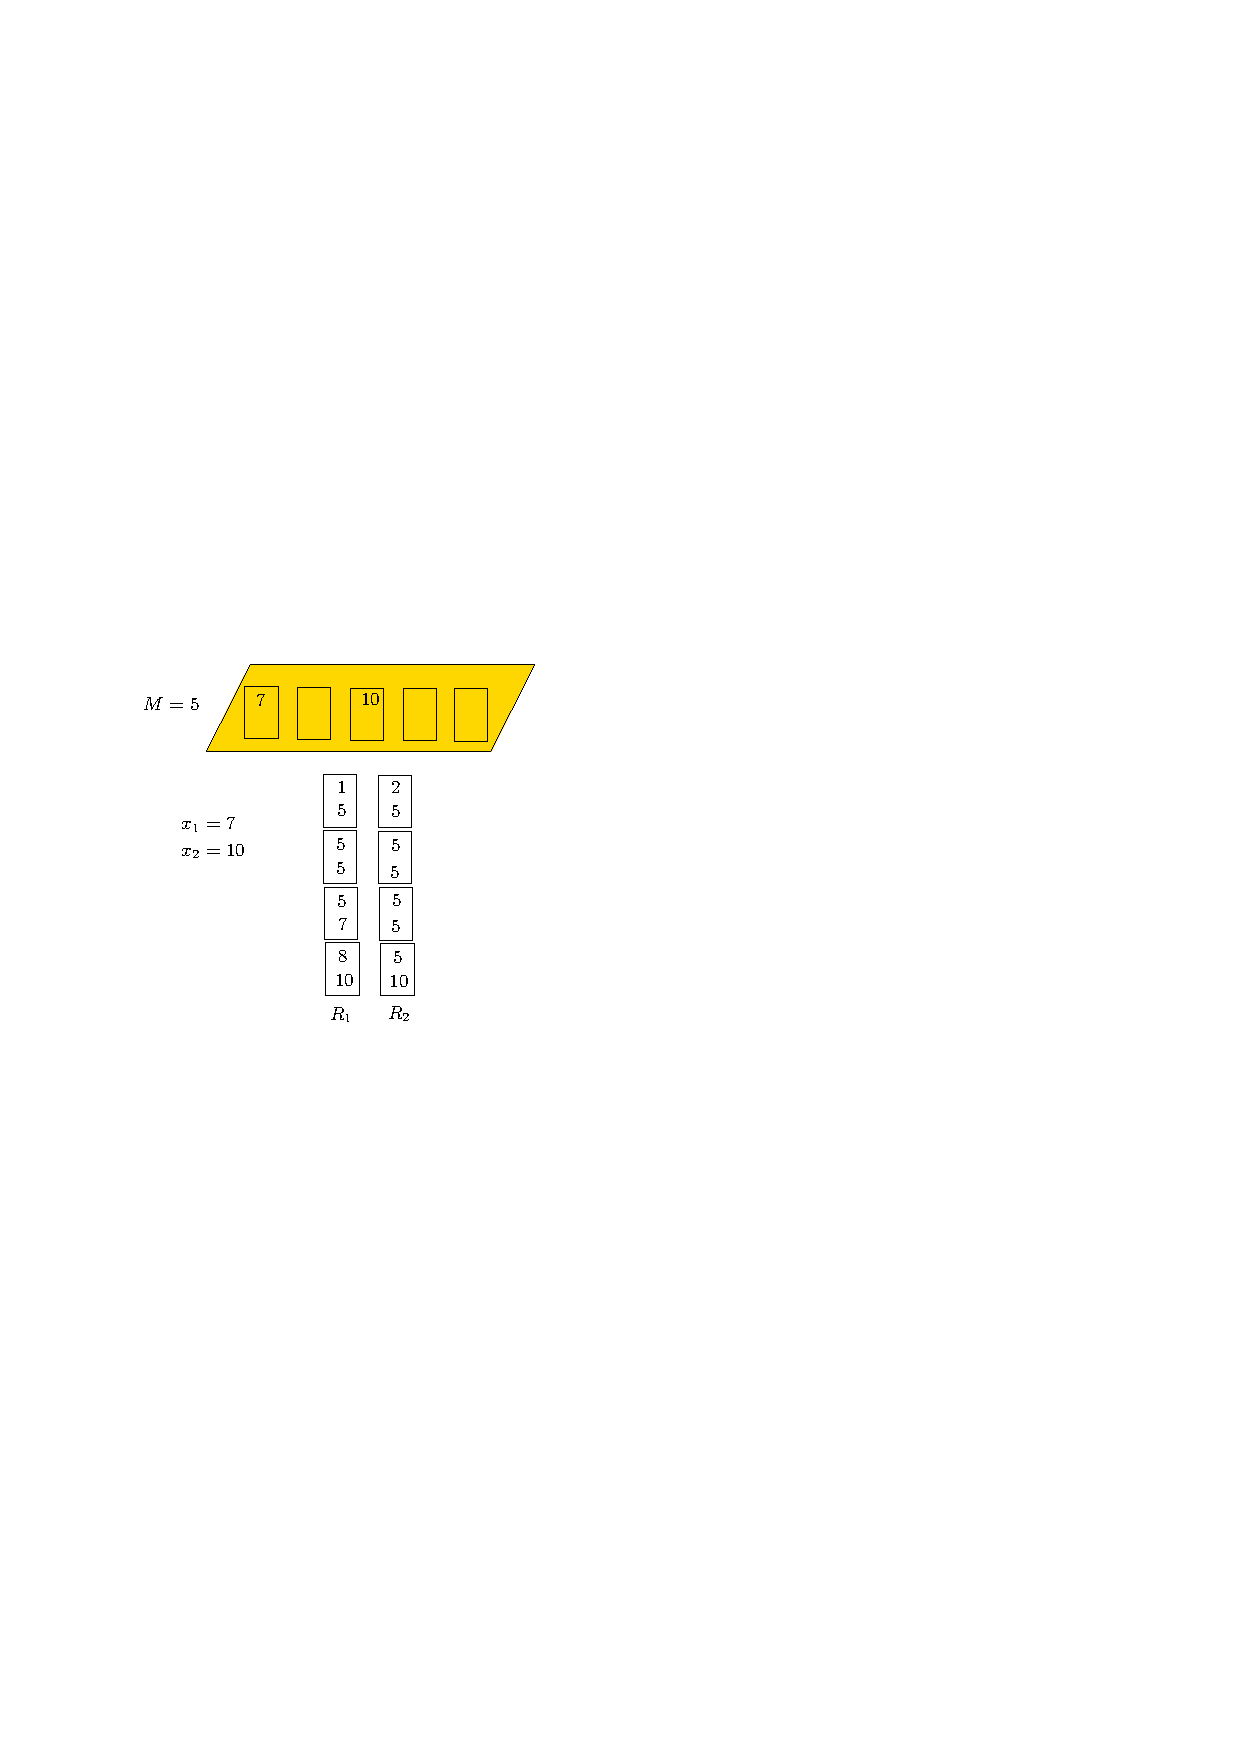
\includegraphics[height=40mm]{./artwork/em-sj5}
    \end{center}

    The algorithm continues in the same fashion until $R_1$ or $R_2$ is exhausted.
}
%-------------------------------------------------------------
\myfrm{
    Every block of $R_1$ and $R_2$ is read exactly once. Hence, Step 2 performs $B_1 + B_2$ I/Os.

    \cbox{blue}{
        The total I/O cost of the sort join algorithm is bounded by $\sort(B_1) + \sort(B_2) + B_1 + B_2$ where $\red{\sort(x)}$ is the I/O cost of sorting $x$ blocks of tuples.
    }

    \cbox{green}{
        In practice, we typically have $B_1 \le M(M-1)$ and $B_2 \le M(M-1)$, in which case the total I/O cost is bounded by $5 (B_1 + B_2)$.
    }

    \cbox{blue}{
        \blue{Remark:} The above analysis has not considered the cost of writing the join result to the disk. If that is necessary, you should add $\red{B_\mit{out}}$ to the I/O cost where $B_\mit{out}$ is the number of blocks needed to store the join result.
    }
}
%-------------------------------------------------------------
\myfrm{
    Here is an interesting question for you:

    \cbox{red}{
        \blue{The 3-Star Join Problem} \\

        $\red{R_1(X, A_1)}$: A relation with attributes $X$ and $A_1$. \\
        $\red{R_2(X, A_2)}$: A relation with attributes $X$ and $A_2$. \\
        $\red{R_3(X, A_3)}$: A relation with attributes $X$ and $A_3$. \\
        $\red{B_i} =$ the number of disk blocks that $R_i$ occupies ($1 \le i \le 3$). \\
        $\red{M} =$ the number of memory blocks.

        \vgap

        If you are to modify the sort-join algorithm to compute $$R_1 \bowtie R_2 \bowtie R_3$$ in $5 (B_1 + B_2 + B_3)$ I/Os, what assumptions would you need?
    }
}
%-------------------------------------------------------------
\myfrm{
    \cbox{yellow}{
        Returning to the binary join problem $R_1(X, Y) \bowtie R_2(X, Z)$, next we outline a refinement of the sort join algorithm that can reduce the I/O cost to $3 (B_1 + B_2)$ when the memory size (i.e., $M$) is reasonably large.

        \vgap

        \blue{Remark:} This content will not be tested.
    }
}
%-------------------------------------------------------------
\myfrm{
    \xmybox{Refined Sort Join}

    %\vgap

    Perform the \bred{initial step} of external sort on $R_1$ (sorting attribute = $X$). \\
    Perform the \bred{initial step} of external sort on $R_2$ (sorting attribute = $X$). \\
    The above needs $2(B_1 + B_2)$ I/Os and yields
    \myitems{
        \item $\red{n_1} = \lc B_1 / M \rc$ \blue{sorted runs} of $R_1$, each having $M$ blocks;
        \item $\red{n_2} = \lc B_2 / M \rc$ \blue{sorted runs} of $R_2$, each having $M$ blocks.
    }

    We assume
    \myitems{
        \item $n_1 + n_2 \le M$;
        \item (\blue{skew condition modified}) for any $X$-value, the tuples of $R_1$ having that $X$-value fit in at most $M - n_2 - n_1$ blocks.
    }

    Under these assumptions, it is possible to scan all the sorted runs synchronously to output $R_1 \bowtie R_2$ directly in $B_1 + B_2$ I/Os \\
    (\blue{think}: how? \blue{hint}: how did you solve the 3-star join problem?).

}
\end{document} 

